%%% LaTeX Template: Article/Thesis/etc. with colored headings and special fonts
%%%
%%% Source: http://www.howtotex.com/
%%% Feel free to distribute this template, but please keep to referal to http://www.howtotex.com/ here.
%%% February 2011
%%%
%%% Modified January 2016 by CDM
%%% Modified/simplified by CTC 2018 - 2023

%%%  Preamble
\documentclass[11pt,letterpaper]{article}
\usepackage[margin=1.0in]{geometry}
\usepackage[T1]{fontenc}
\usepackage[bitstream-charter]{mathdesign}
\usepackage[latin1]{inputenc}					
\usepackage{amsmath}						
\usepackage{xcolor}
\usepackage{cite}
\usepackage{hyphenat}
\usepackage{graphicx}
\usepackage{float}
\usepackage{subfigure}
\usepackage{sectsty}
\usepackage[compact]{titlesec} 
\usepackage[tablegrid]{vhistory}
\usepackage{pbox}
\allsectionsfont{\color{accentcolor}\scshape\selectfont}

%%% Definitions
%%%%%%%%%%%%%%%%%%%%%%%%%%%%%%%%%%%%%%%%%%%%%%%%%%
% Change me to fit your team/semester information
\definecolor{accentcolor}{rgb}{0.0,0.0,0.5} 
\newcommand{\teamname}{Team TLC}               %just to fill the line
\newcommand{\productname}{Roam\_Bot}
\newcommand{\coursename}{CSE 4316: Senior Design I}
\newcommand{\semester}{Fall 2024}
\newcommand{\docname}{Architectural Design Specification}
\newcommand{\department}{Department of Computer Science \& Engineering}
\newcommand{\university}{The University of Texas at Arlington}
\newcommand{\authors}{Abubakar Kassim \\ Andrew Howard \\ Christopher Davis \\ Madison Gage \\ Raya Sultan \\}

%%% Headers and footers
\usepackage{fancyhdr}
	\pagestyle{fancy}						% Enabling the custom headers/footers
\usepackage{lastpage}	
	% Header (empty)
	\lhead{}
	\chead{}
	\rhead{}
	% Footer
	\lfoot{\footnotesize \teamname \ - \semester}
	\cfoot{}
	\rfoot{\footnotesize page \thepage\ of \pageref{LastPage}}	% "Page 1 of 2"
	\renewcommand{\headrulewidth}{0.0pt}
	\renewcommand{\footrulewidth}{0.4pt}

%%% Change the abstract environment
\usepackage[runin]{abstract}			% runin option for a run-in title
%\setlength\absleftindent{30pt}			% left margin
%\setlength\absrightindent{30pt}		% right margin
\abslabeldelim{\quad}	
\setlength{\abstitleskip}{-10pt}
\renewcommand{\abstractname}{}
\renewcommand{\abstracttextfont}{\color{accentcolor} \small \slshape}	% slanted text

%%% Start of the document
\begin{document}

%%% Cover sheet
{\centering \huge \color{accentcolor} \sc \textbf{\department \\ \university} \par} % department/university info
\vspace{1 in}
{\centering \huge \color{accentcolor} \sc \textbf{\docname \\ \coursename \\ \semester} \par} % doc/semester info
\vspace{0.1 in} % spacing before cover sheet image
%%%%%%%%%%%%%%%%%%%%%%%%%%%%%%%%%%%%%%%%%%%%%%%%%%%%%%%%%%%%%%%%%%%%%%%%%%%%
%   Change the graphic here. Put your image in the 'images' folder
%   and update the name from 'images/test_image' to your image name
\begin{figure}[h!]
	\centering
   	
\includegraphics[width=0.60\textwidth]{images/final_logo-removebg-preview.png}
\end{figure}
\vspace{0.1 in} % spacing after cover sheet image, before team/product info
{\centering \huge \color{accentcolor} \sc \textbf{\teamname \\ \productname} \par}
\vspace{0.1 in} % spacing before team members
{\centering \large \sc \textbf{\authors} \par}
\newpage


%\vspace{1 in}
%\centerline{January 13th, 2012}
%\newpage

%%% Revision History
%%%%%%%%%%%%%%%%%%%%%%%%%%%%%%%%%%%%%%%%%%%%%%%%%%%%%%%%%%%%%%%%%
% Each '\vhEntry' begins a new version entry, and each {} is a 
% column. Update this to reflect your version history.
\begin{versionhistory}
  	\vhEntry{0.1}{11.05.2024}{CD}{document creation}
        \vhEntry{0.2}{11.19.2024}{CD}{added the introduction}
        \vhEntry{0.3}{11.19.2024}{MG}{created architecture diagram}
  	\vhEntry{0.4}{11.20.2024}{AH}{added movement subsystems}
  	\vhEntry{0.5}{11.24.2024}{AK}{added pathfinding subsystems}
        \vhEntry{0.6}{11.24.2024}{RS}{added interface subsystems}
  	\vhEntry{1.0}{11.25.2024}{CD|RS|MG|AK|AH}{official release}
\end{versionhistory}
\newpage

%%% Table of contents
\setcounter{tocdepth}{2}
\tableofcontents
\newpage

%%% List of figures and tables (optional)
\listoffigures
\listoftables
\newpage

%%% Document sections
% The \section command creates a section, assigns it a number and gives it the title in the braces.
% The \input command inserts the contents of the text file indicated in the braces.
\section{Introduction}
% Your introduction should provide a brief overview of the product concept and a reference to the requirement specification and architectural design documents in 1 or 2 paragraphs. The purpose is to provide the reader with the location of relevant background material that lead to the design details presented in this document.

The RoamBot should assist with learning to implement autonomous system software through real test simulations. This will be achieved using actual robotic systems. The overall design is controlled by a Raspberry Pi, which acts as the host connecting the different components of the rover. The first section describes the rover's motion and functionality. The second section entails the interface which allows users to upload their algorithm or manually control the rover. The third section is about the path-finding function, which dictates where the rover can move with the use of LIDAR and other sensors.

\newpage
\section{System Overview}
This section should reintroduce the full data flow diagram from the architectural specification, and discuss at a high level the purpose of each layer. You do not need to include a subsection for each layer, a 1 - 2 paragraph recap is sufficient.

\begin{figure}[h!]
	\centering
 	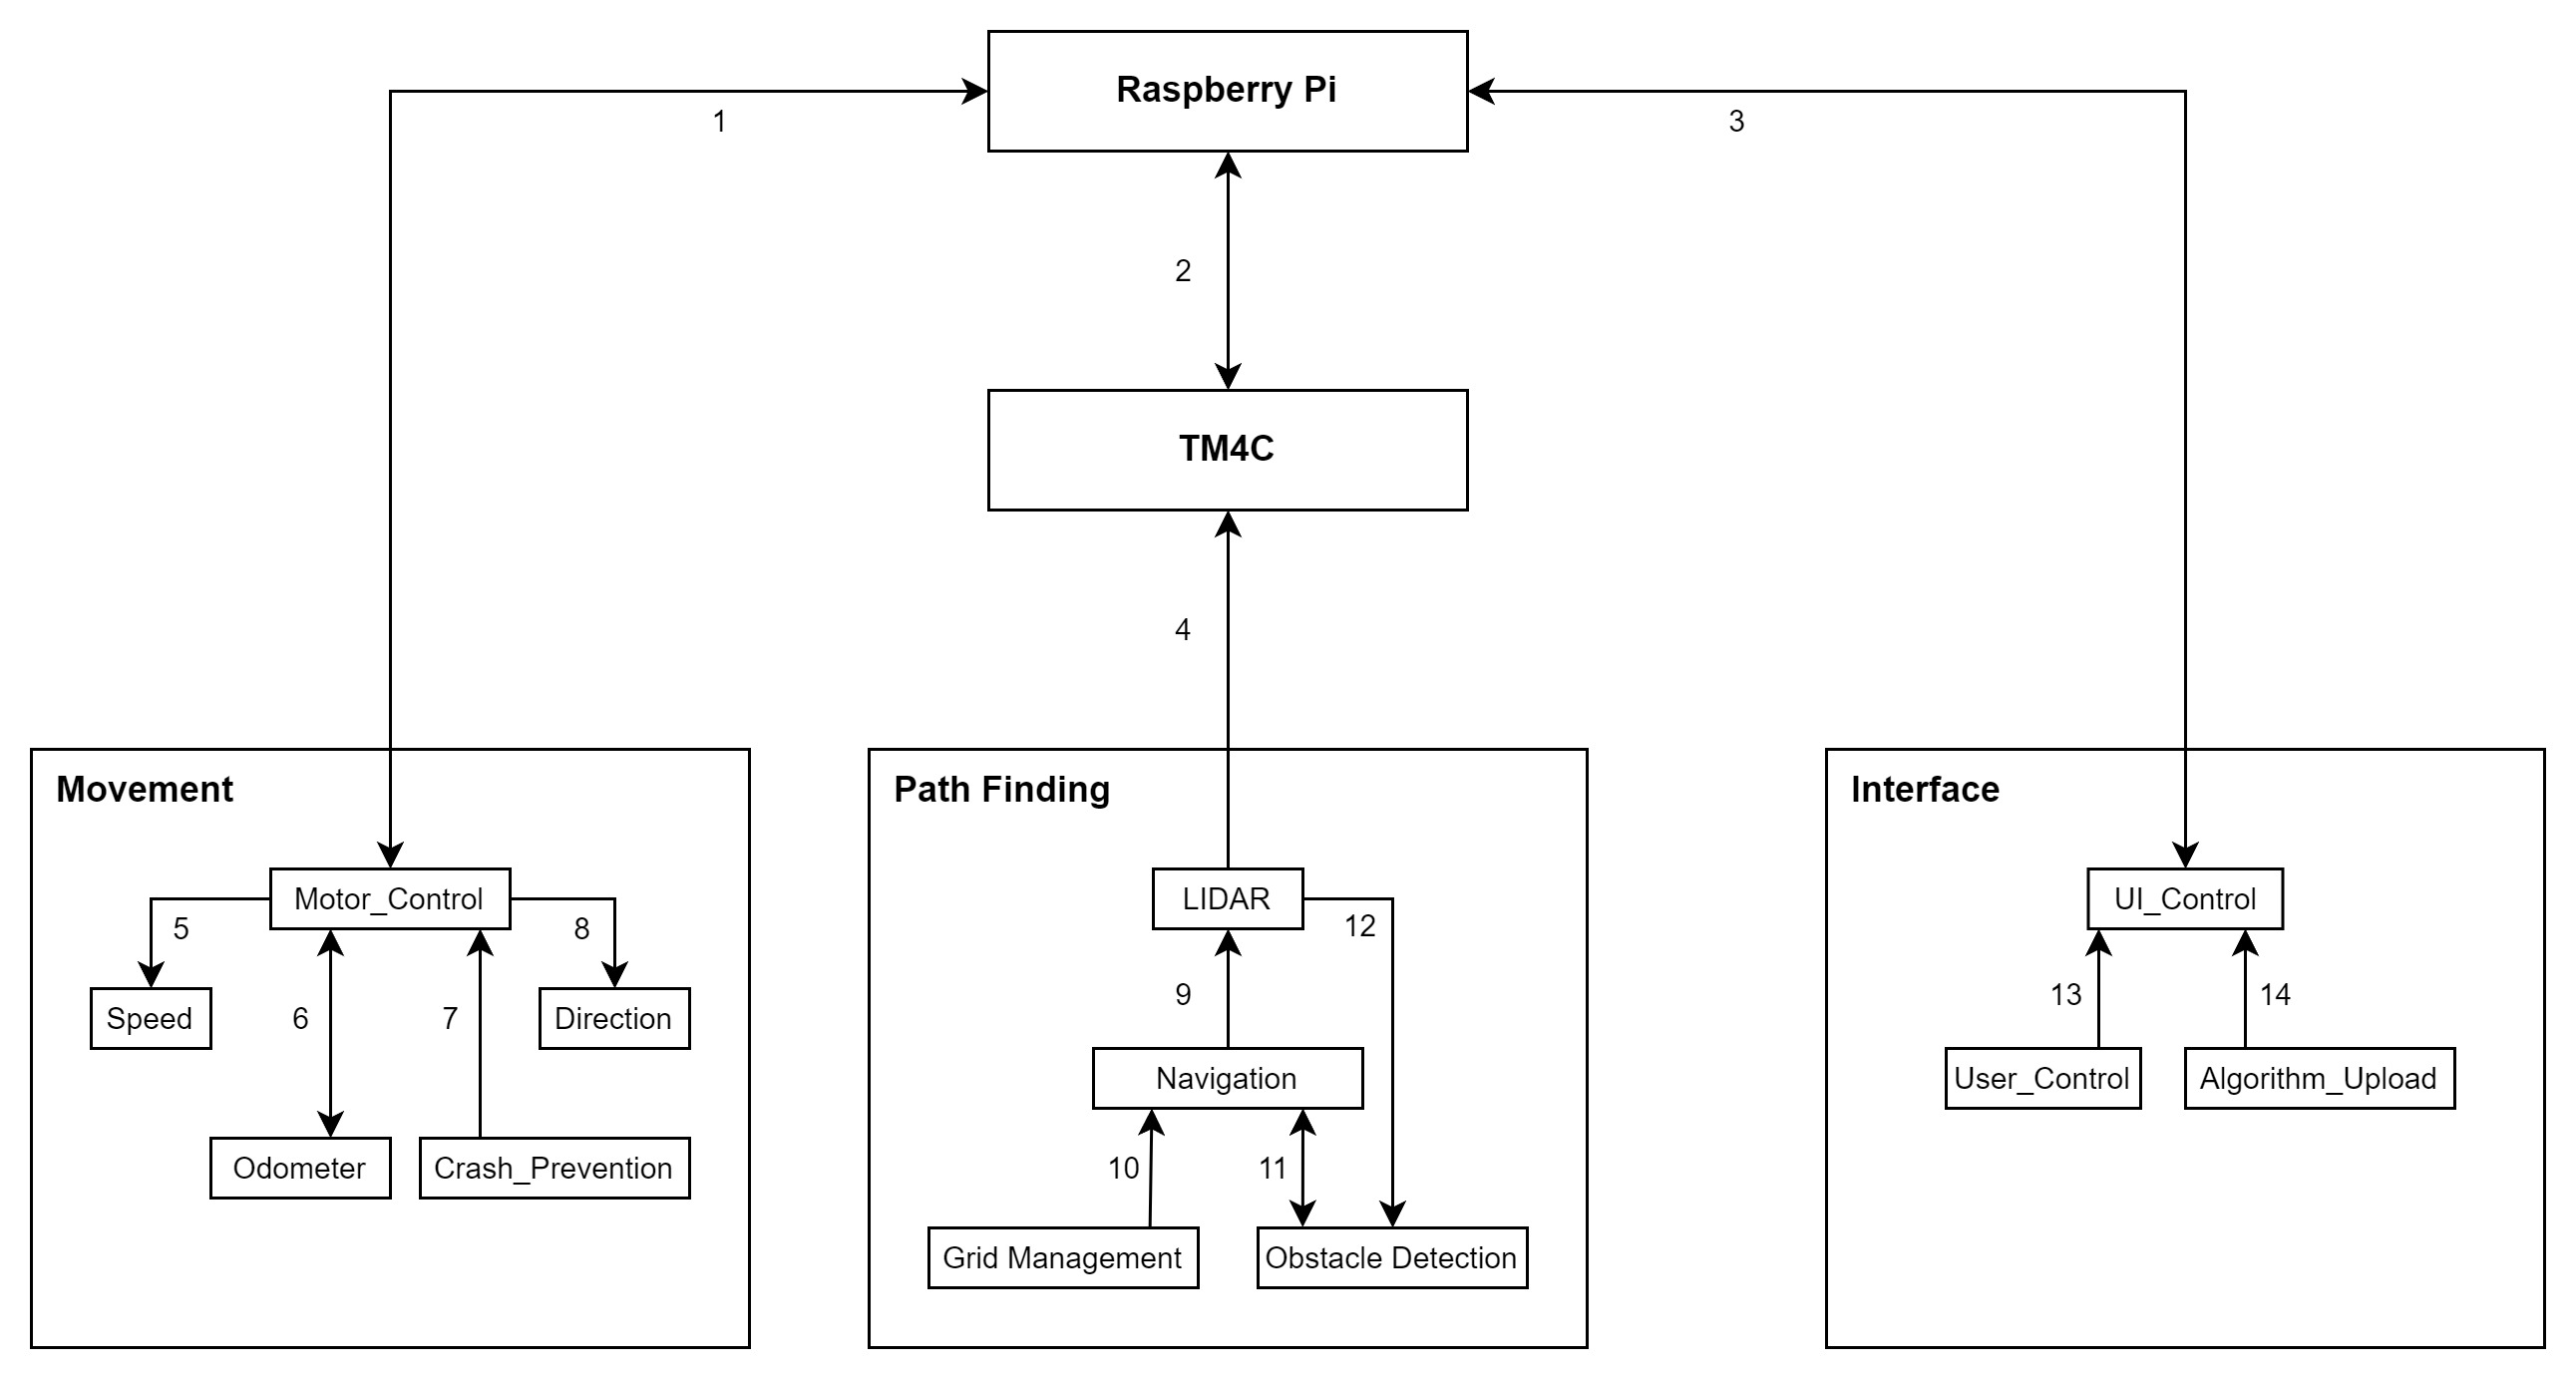
\includegraphics[width=0.90\textwidth]{images/data_flow}
 \caption{System architecture}
\end{figure}

\newpage
\section{Subsystem Definitions \& Data Flow}
% This section breaks down your layer abstraction to another level of detail. Here you grapically represent the logical subsytems that compose each layer and show the interactions/interfaces between those subsystems. A subsystem can be thought of as a programming unit that implements one of the major functions of the layer. It, therefore, has data elements that serve as source/sinks for other subsystems. The logical data elements that flow between subsystems need to be explicitly defined at this point, beginning with a data flow-like diagram based on the block diagram.

%%%%%%%%%%%%%%%%%%%%%%%%%%%%%%%%%%%%%%%%%%%%%%%%%%%%%%%%%%%%%%%%%%%%%%%%%%%%
%   Change the graphic here. Put your image in the 'images' folder
%   and update the name from 'images/test_image' to your image name
\begin{figure}[h!]
	\centering
 	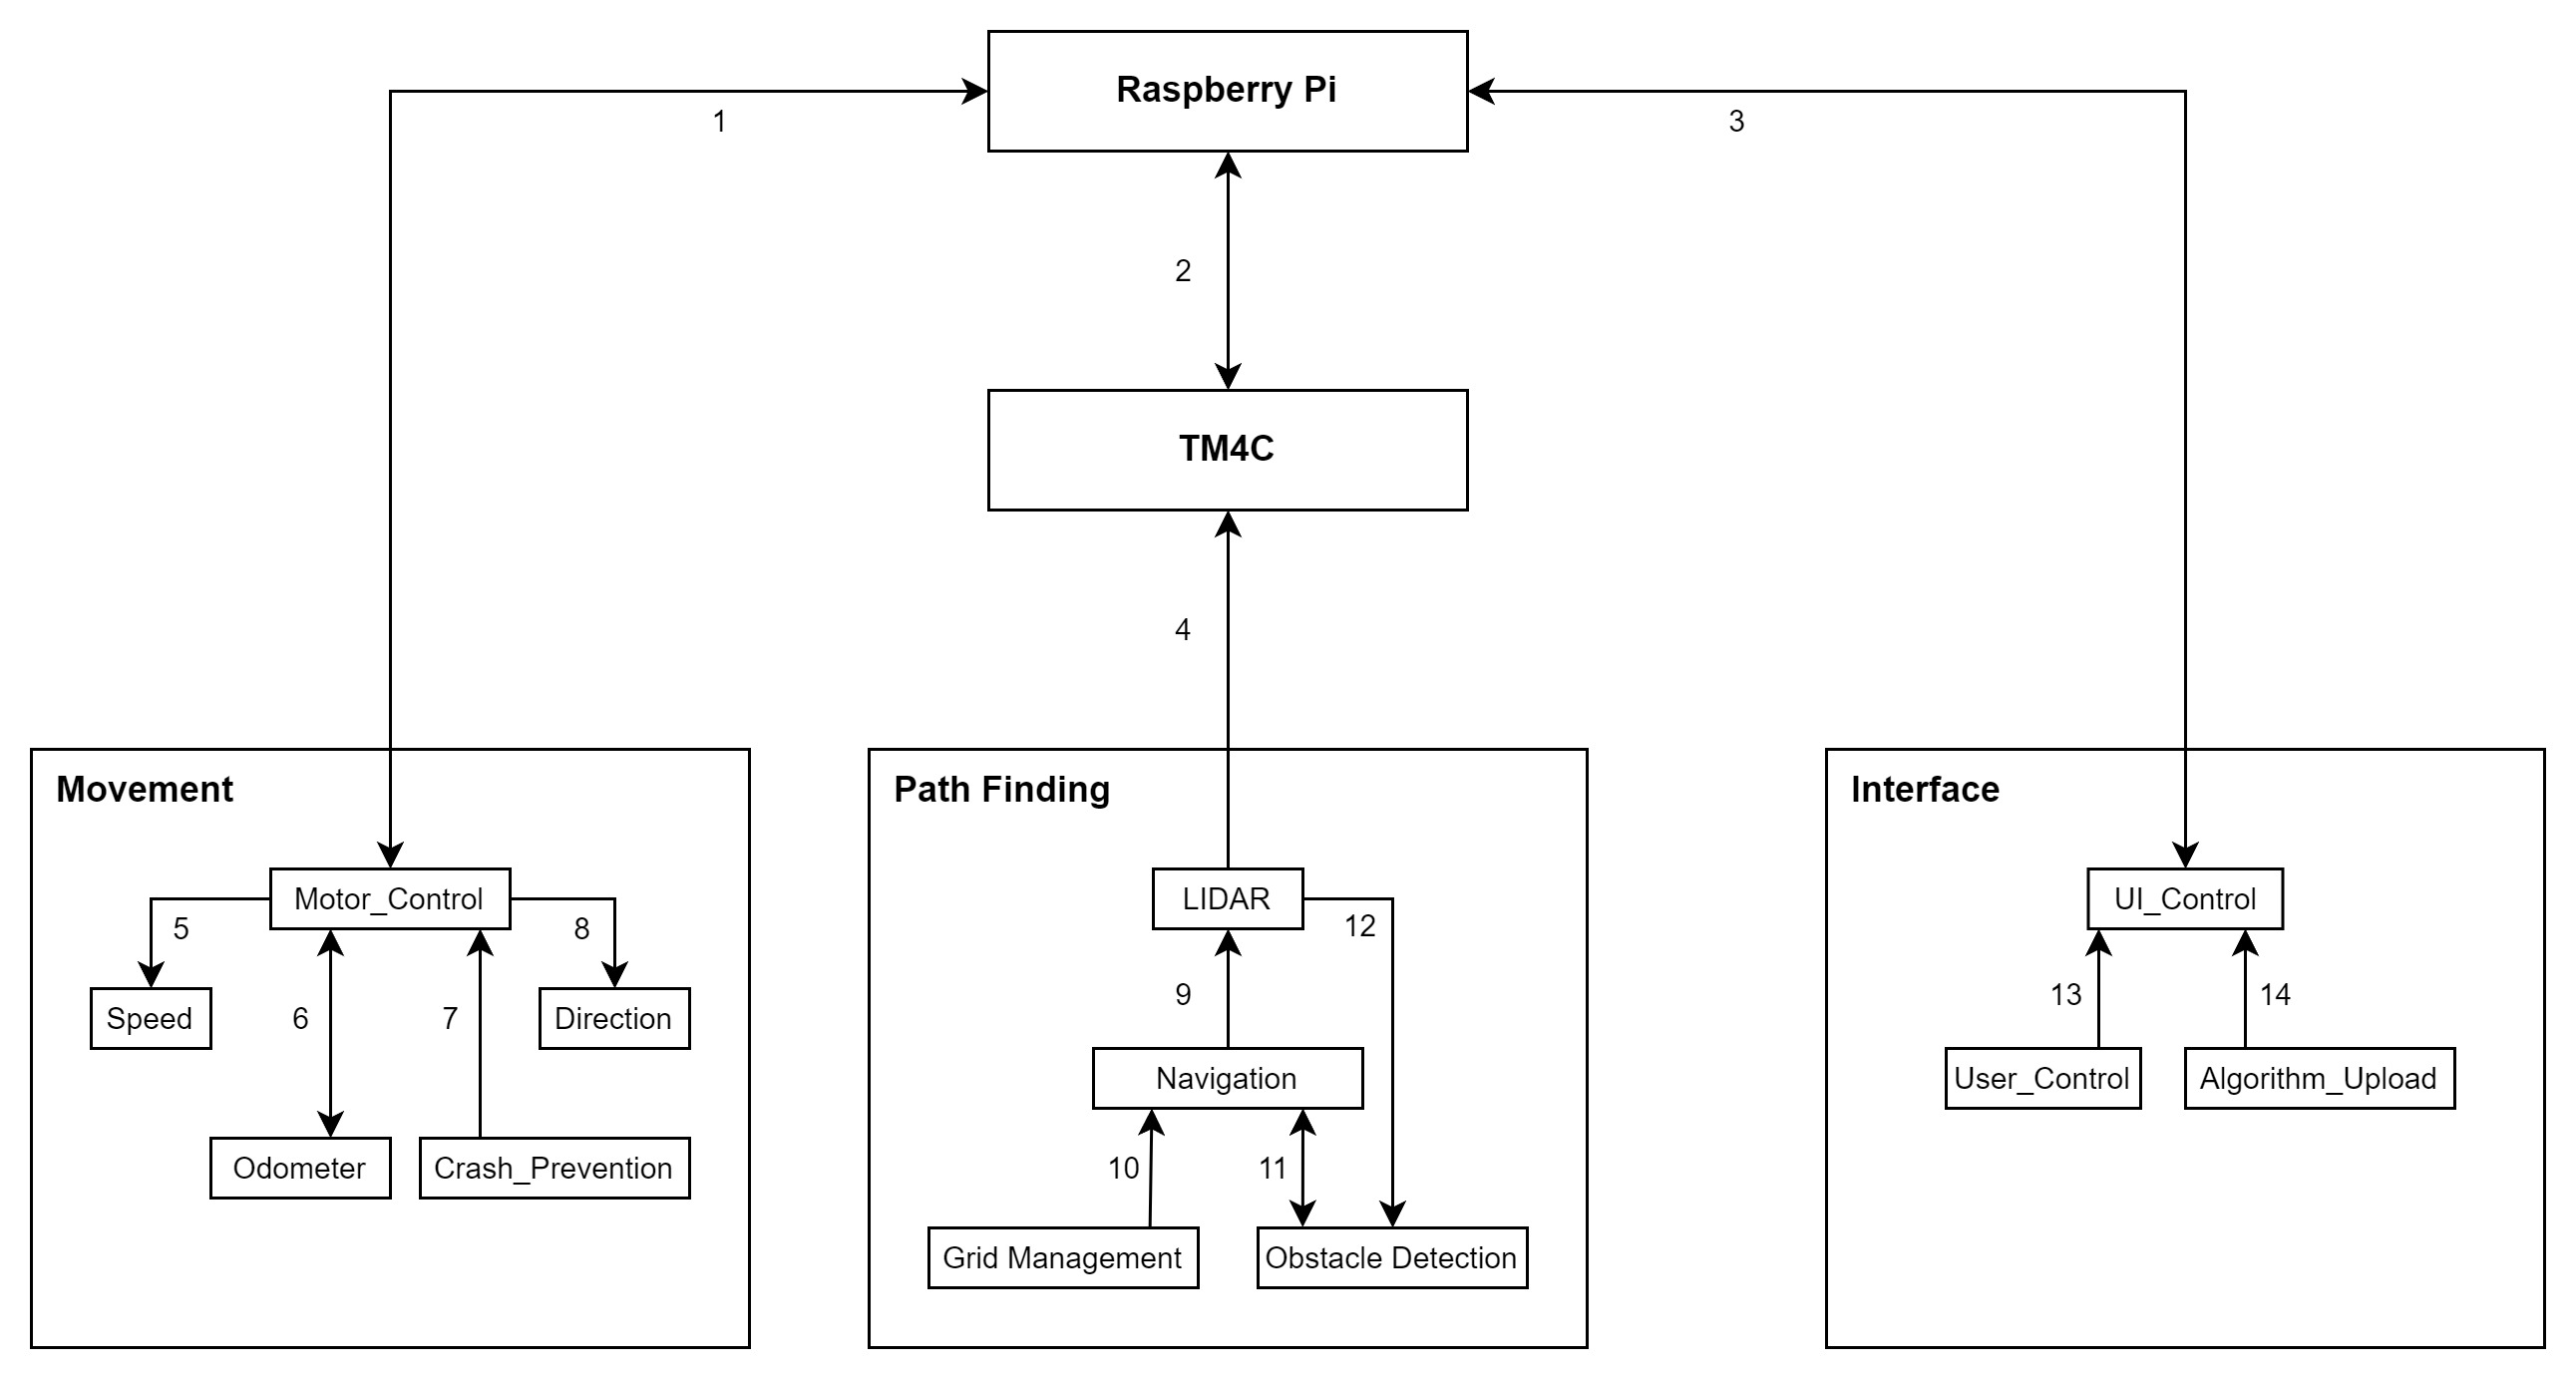
\includegraphics[width=\textwidth]{images/data_flow}
 \caption{A simple data flow diagram} % Be sure to change the caption!
\end{figure}

\newpage
\section{Movement Subsystems}
% In this section, the layer is described in some detail in terms of its specific subsystems. Describe each of the layers and its subsystems in a separate chapter/major subsection of this document. The content of each subsystem description should be similar. Include in this section any special considerations and/or trade-offs considered for the approach you have chosen.

%%%%%%%%%%%%%%%%%%%%%%%%%%%%%%%%%%%%%%%%%%%%%%%%%%%%%%%%%%%%%%%%%%%%%%%%%%%%

\subsection{Speed Control}
% This section should be a general description of a particular subsystem for the given layer. For most subsystems, an extract of the architectural block diagram with data flows is useful. This should consist of the subsystem being described and those subsystems with which it communicates.
The speed control subsystem manages the power of each motor to maintain a specific set speed. It receives feedback from the odometer and crash prevention to ensure safe operation.

%   Change the graphic here. Put your image in the 'images' folder
%   and update the name from 'images/test_image' to your image name
\begin{figure}[h!]
	\centering
 	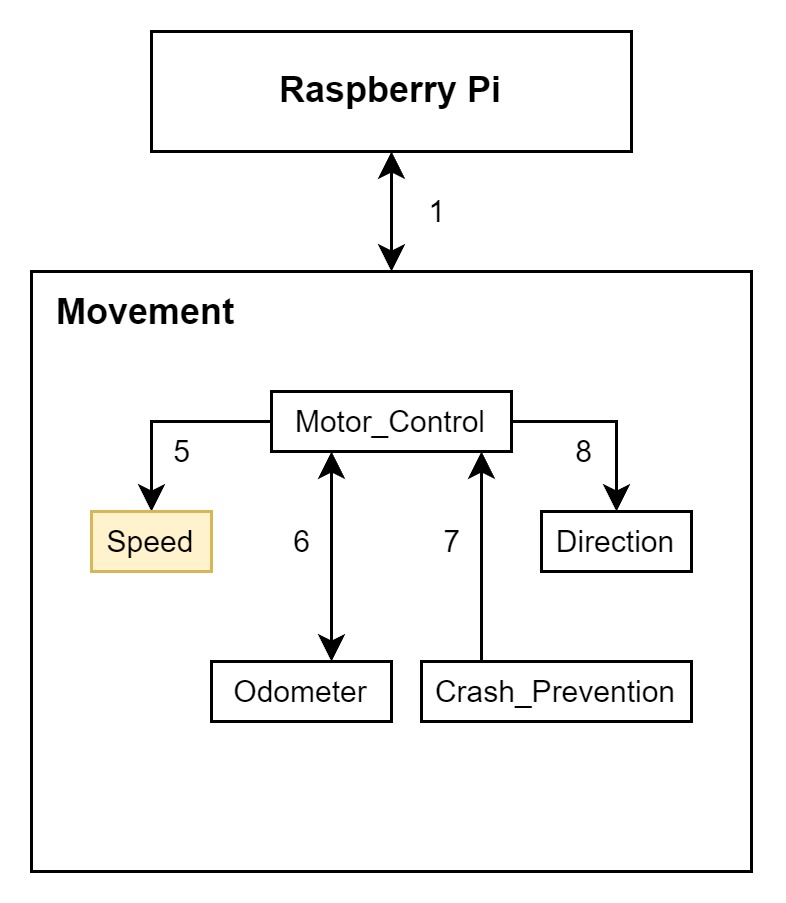
\includegraphics[width=0.45\textwidth]{images/movement/speed.jpg}
 \caption{Movement Subsystem - Speed Control} % Be sure to change the caption
\end{figure}

\subsubsection{Assumptions}
% Any assumptions made in the definition of the subsystem should be listed and described. Pay particular attention to assumptions concerning interfaces and interactions with other layers.
The motor driver supports PWM input to control motor speed. The odometer feedback is accurate within 10\% from wheel encoder measurements \cite{Zhang2020}. Communication latency between the TM4C and Raspberry Pi isn't noticeable for real-time feedback.

\subsubsection{Responsibilities}
% Each of the responsibilities/features/functions/services of the subsystem as identified in the architectural summary must be expanded to more detailed responsibilities. These responsibilities form the basis for the identification of the finer-grained responsibilities of the layer's internal subsystems. Clearly describe what each subsystem does.
Adjust motor PWM signals to match the target speed set. Monitor odometer feedback to ensure the actual speed matches the desired speed. Stop the speed if a collision is detected.

\subsubsection{Subsystem Interfaces}
% Each of the inputs and outputs for the subsystem are defined here. Create a table with an entry for each labeled interface that connects to this subsystem. For each entry, describe any incoming and outgoing data elements will pass through this interface.

\begin {table}[H]
\caption {Movement Subsystem - Speed Control} 
\begin{center}
    \begin{tabular}{ | p{1cm} | p{6cm} | p{3cm} | p{3cm} |}
    \hline
    ID & Description & Inputs & Outputs \\ \hline
    \#5 & Pulse Width Modulation (PWM) & Power In & N/A \\ \hline
    \end{tabular}
\end{center}
\end{table}

\newpage

%%%%%%%%%%%%%%%%%%%%%%%%%%%%%%%%%%%%%%%%%%%%%%%%%%%%%%%%%%%%%%%%%%%%%%%%%%%%%%%%%%

\subsection{Direction Control}
The direction control subsystem manages the robot's steering by adjusting the motor signals for the left and right wheels. It receives feedback from the steering sensors and ensures the rover follows the correct path.

\begin{figure}[h!]
	\centering
 	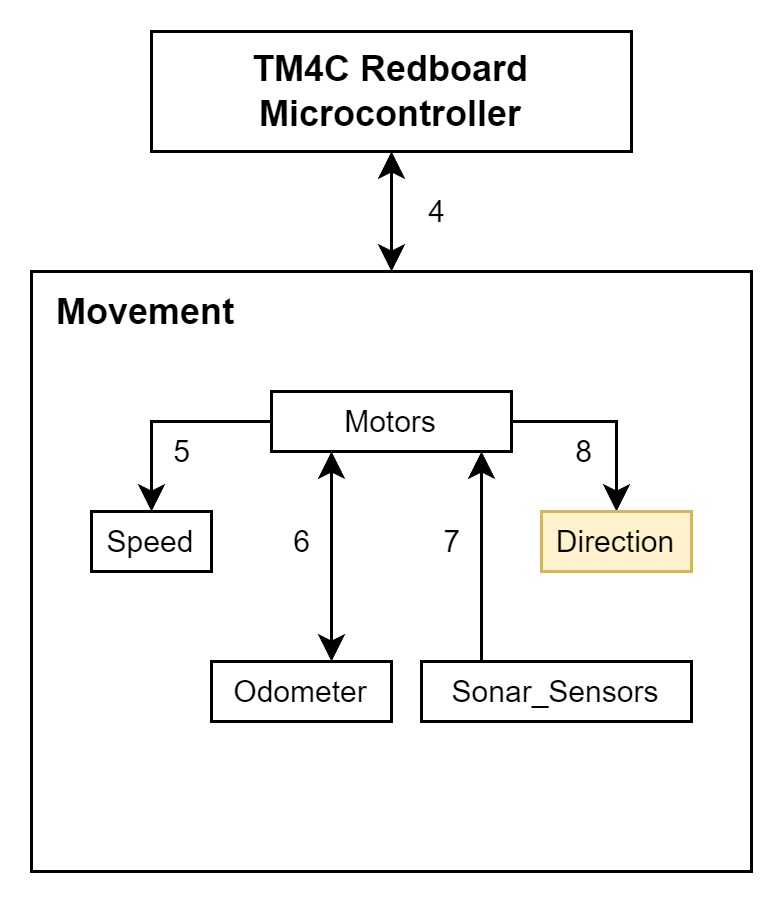
\includegraphics[width=0.45\textwidth]{images/movement/direction.jpg}
 \caption{Movement Subsystem - Direction Control} % Be sure to change the caption
\end{figure}

\subsubsection{Assumptions}
The motor driver supports PWM input to control motor direction. The steering feedback system is accurate within 5\% from LIDAR measurements \cite{Epton2012}. Communication latency between the TM4C and Raspberry Pi is minimal for real-time control.

\subsubsection{Responsibilities}
Adjust motor PWM signals to steer the robot in the desired direction. Monitor steering feedback to ensure the robot is following the intended path. Correct any misalignment detected by the steering sensors.

\subsubsection{Subsystem Interfaces}

\begin {table}[H]
\caption {Movement Subsystem - Direction Control} 
\begin{center}
    \begin{tabular}{ | p{1cm} | p{6cm} | p{3cm} | p{3cm} |}
    \hline
    ID & Description & Inputs & Outputs \\ \hline
    \#8 & Pulse Width Modulation (PWM) & Power In & N/A \\ \hline
    \end{tabular}
\end{center}
\end{table}

\newpage

%%%%%%%%%%%%%%%%%%%%%%%%%%%%%%%%%%%%%%%%%%%%%%%%%%%%%%%%%%%%%%%%%%%%%%%%%%%%%%%%%%

\subsection{Motor Control}
The motor control subsystem manages the power supplied to the motors to achieve the desired movement. It receives feedback from the motor encoders and adjusts the motor signals to control both speed and direction.

\begin{figure}[h!]
	\centering
 	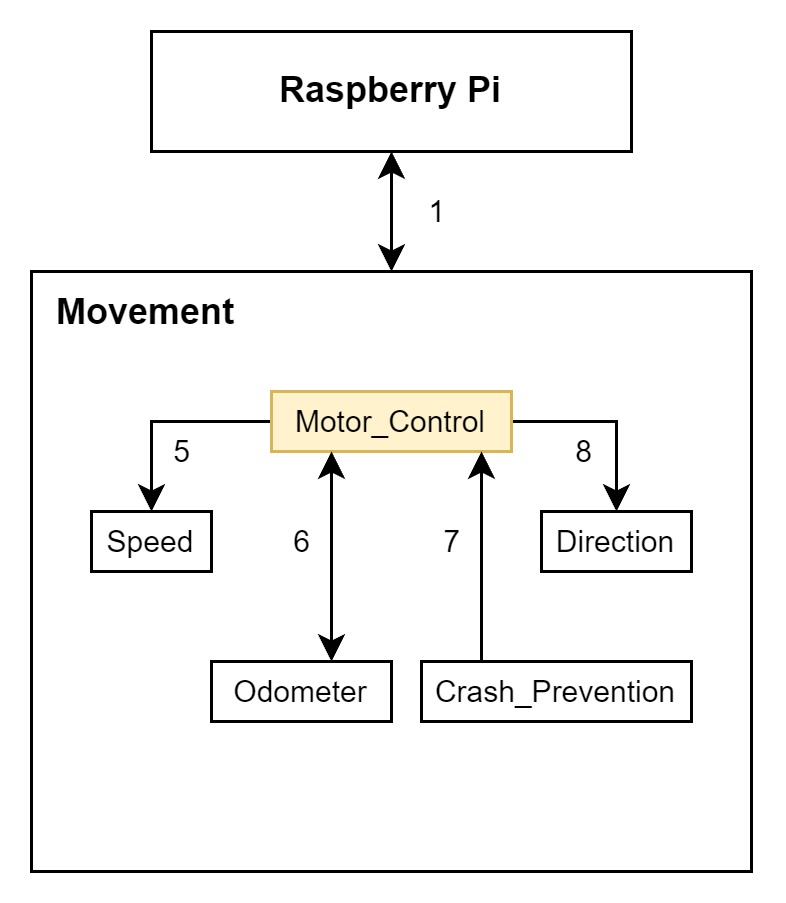
\includegraphics[width=0.45\textwidth]{images/movement/motor_control.jpg}
 \caption{Movement Subsystem - Motor Control} % Be sure to change the caption
\end{figure}

\subsubsection{Assumptions}
The motor driver supports both PWM and direction control signals to drive motor speed and direction \cite{DimensionEngineeringSabertooth2x25}. The motor encoders provide accurate feedback to control speed and direction adjustments. Communication latency between the TM4C and Raspberry Pi does not impact real-time motor control.

\subsubsection{Responsibilities}
Control motor power to achieve the desired speed and direction. Monitor motor feedback to ensure correct operation and make adjustments when necessary. Handle error states, such as motor stall or failure, and stop the motors if a critical fault is detected.

\subsubsection{Subsystem Interfaces}

\begin{table}[H]
\caption{Movement Subsystem - Motor Control} 
\begin{center}
    \begin{tabular}{ | p{0.8cm} | p{6cm} | p{4cm} | p{3cm} |}
    \hline
    ID & Description & Inputs & Outputs  \\ \hline
    \#5 & Pulse Width Modulation (PWM) & N/A & Power Output \\ \hline
    \#6 & General Purpose Input Output (GPIO) & Odometer Feedback  & Odometer Control \\ \hline
    \#7 & General Purpose Input Output (GPIO) & Crash Detect & N/A \\ \hline
    \#8 & Pulse Width Modulation (PWM) & N/A & Power Output \\ \hline
    \end{tabular}
\end{center}
\end{table}

\newpage

%%%%%%%%%%%%%%%%%%%%%%%%%%%%%%%%%%%%%%%%%%%%%%%%%%%%%%%%%%%%%%%%%%%%%%%%%%%%%%%%%%

\subsection{Odometer}
The odometer subsystem is responsible for measuring the distance traveled by the vehicle. It provides feedback to the motor control subsystem to help adjust the speed and ensure accurate movement over time.

\begin{figure}[h!]
	\centering
 	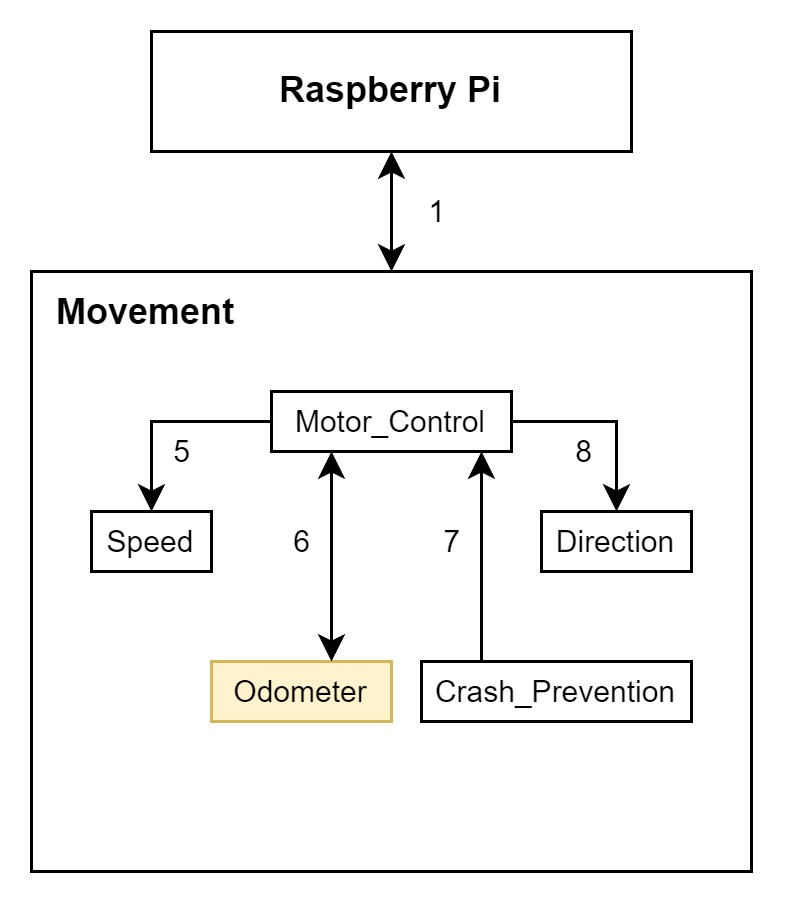
\includegraphics[width=0.45\textwidth]{images/movement/odometer.jpg}
 \caption{Movement Subsystem - Odometer} % Be sure to change the caption
\end{figure}

\subsubsection{Assumptions}
The odometer system uses wheel encoders and LIDAR to measure the distance traveled. The feedback is accurate within 10\% for distance measurement \cite{Zhang2020} \cite{Epton2012}. The odometer data is updated in real time, with no significant communication delays between the TM4C and Raspberry Pi affecting its accuracy.

\subsubsection{Responsibilities}
Measure the distance traveled by the vehicle based on wheel rotations. Provide real-time feedback to the motor control subsystem to adjust the speed accordingly. Alert the system if abnormal readings are detected, such as wheel slippage or encoder malfunction.

\subsubsection{Subsystem Interfaces}

\begin{table}[H]
\caption{Movement Subsystem - Odometer} 
\begin{center}
    \begin{tabular}{ | p{0.8cm} | p{6cm} | p{3cm} | p{4cm} |}
    \hline
    ID & Description & Inputs & Outputs  \\ \hline
    \#6 & General Purpose Input Output (GPIO) & Odometer Control & Odometer Feedback \\ \hline
    \end{tabular}
\end{center}
\end{table}

\newpage

%%%%%%%%%%%%%%%%%%%%%%%%%%%%%%%%%%%%%%%%%%%%%%%%%%%%%%%%%%%%%%%%%%%%%%%%%%%%%%%%%%

\subsection{Crash Detection}
The crash detection subsystem is responsible for identifying any potential collisions or obstacles in the vehicle's path. It monitors sensor data to detect obstacles or sudden changes in velocity that may indicate a crash or near-crash event.

\begin{figure}[h!]
	\centering
 	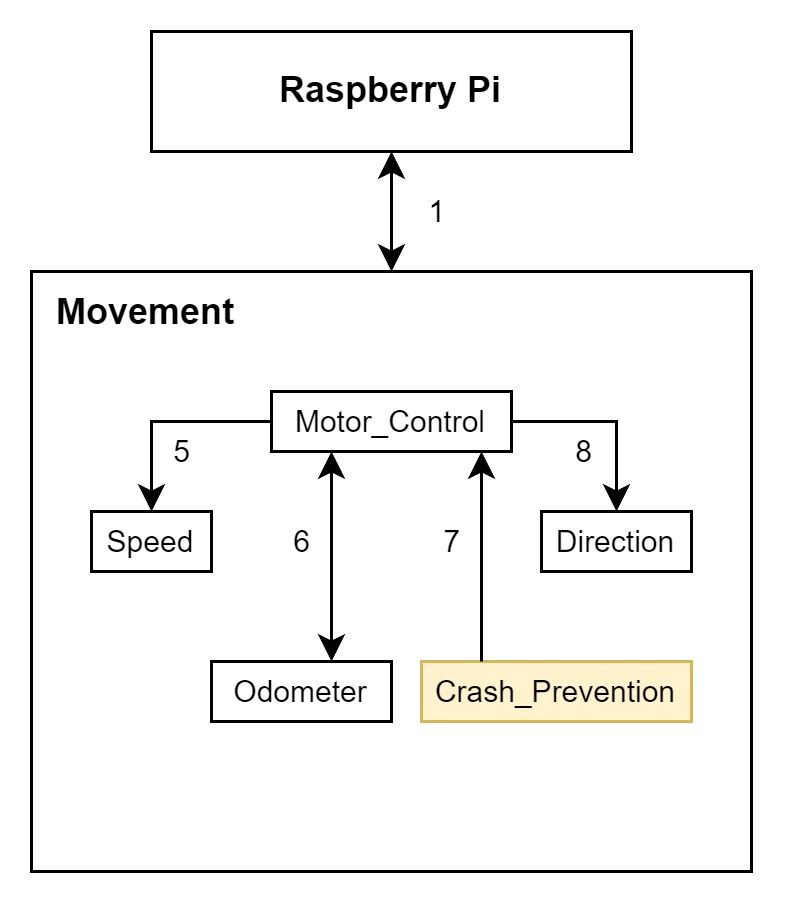
\includegraphics[width=0.45\textwidth]{images/movement/crash_prevention.jpg}
 \caption{Movement Subsystem - Crash Detection} % Be sure to change the caption
\end{figure}

\subsubsection{Assumptions}
The crash detection system uses a combination of proximity sensors and accelerometers to detect obstacles and sudden impacts \cite{Hassan2012}.The sensor system is accurate within a range of 5 cm for obstacle detection, and the accelerometers can detect changes in velocity. Communication latency between the TM4C and Raspberry Pi is minimal and does not affect real-time collision detection.

\subsubsection{Responsibilities}
Monitor sensor data to detect any obstacles or sudden changes in velocity. Alert the motor control subsystem to stop or adjust the vehicle's movement if a crash is detected. Ensure that the vehicle responds promptly to prevent further damage or injury in case of a collision.

\subsubsection{Subsystem Interfaces}

\begin {table}[H]
\caption {Movement Subsystem - Crash Detection} 
\begin{center}
    \begin{tabular}{ | p{1cm} | p{6cm} | p{3cm} | p{3cm} |}
    \hline
    ID & Description & Inputs & Outputs \\ \hline
    \#7 & General Purpose Input Output (GPIO) & Crash Detect & N/A \\ \hline
    \end{tabular}
\end{center}
\end{table}

\newpage

\newpage
\section{Pathfinding Subsystems}
% In this section, the layer is described in some detail in terms of its specific subsystems. Describe each of the layers and its subsystems in a separate chapter/major subsection of this document. The content of each subsystem description should be similar. Include in this section any special considerations and/or trade-offs considered for the approach you have chosen.

The pathfinding subsystem manages the components or modules within a larger pathfinding system that handles specific aspects of the 

\subsection{Static Map Subsystem}
The Static Map subsystem allows the display of the LiDAR range as a grid of cells and allows them to be marked as either traversable or non-traversable, as needed.

% This section should be a general description of a particular subsystem for the given layer. For most subsystems, an extract of the architectural block diagram with data flows is useful. This should consist of the subsystem being described and those subsystems with which it communicates.


%%%%%%%%%%%%%%%%%%%%%%%%%%%%%%%%%%%%%%%%%%%%%%%%%%%%%%%%%%%%%%%%%%%%%%%%%%%%
%   Change the graphic here. Put your image in the 'images' folder
%   and update the name from 'images/test_image' to your image name
\begin{figure}[h!]
	\centering
 	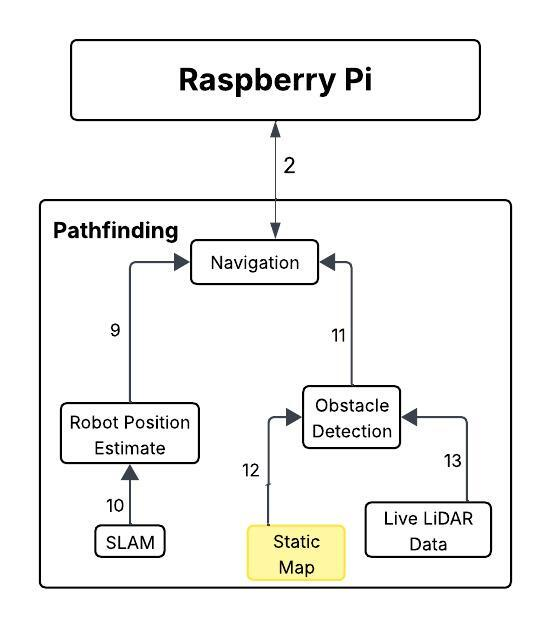
\includegraphics[width=0.80\textwidth]{images/pathfinding 2/Data_Flow_StaticMap.jpeg}
 \caption{Pathfinding Subsystem - Static Map} % Be sure to change the caption.
\end{figure}

\subsubsection{Assumptions}
% Any assumptions made in the definition of the subsystem should be listed and described. Pay particular attention to assumptions concerning interfaces and interactions with other layers.

Static Map assumes that the Obstacle Detection will be functional, and there will not be dynamic obstacles or other movement during pathfinding.
\subsubsection{Responsibilities}
% Each of the responsibilities/features/functions/services of the subsystem as identified in the architectural summary must be expanded to more detailed responsibilities. These responsibilities form the basis for the identification of the finer-grained responsibilities of the layer's internal subsystems. Clearly describe what each subsystem does.

The static map creates a map using the SlamTec LiDAR to than feed into the Obstacle Detection Subystem, so that it can create a costmap.
\subsubsection{Subsystem Interfaces}
% Each of the inputs and outputs for the subsystem are defined here. Create a table with an entry for each labelled interface that connects to this subsystem. For each entry, describe any incoming and outgoing data elements will pass through this interface.

\begin {table}[H]
\caption {Pathfinding Subsystem - Static Map} 
\begin{center}
    \begin{tabular}{ | p{1.2cm} | p{6cm} | p{3cm} | p{3cm} |}
    \hline
    ID & Description & Inputs & Outputs \\ \hline
    \#12 & Data converts Laser Scan into Map & \pbox{3cm}{N/A} & \pbox{3cm}{Map (.yaml file) }  \\ \hline

    \end{tabular}
\end{center}
\end{table}

\newpage

\subsection{Obstacle Detection Subsystems}
The obstacle detection subsystem is designed to process feedback from the LiDAR, identifying objects within its range and marking them as impassable when necessary.
%%%%%%%%%%%%%%%%%%%%%%%%%%%%%%%%%%%%%%%%%%%%%%%%%%%%%%%%%%%%%%%%%%%%%%%%%%%%
%   Change the graphic here. Put your image in the 'images' folder
%   and update the name from 'images/test_image' to your image name
\begin{figure}[h!]
	\centering
 	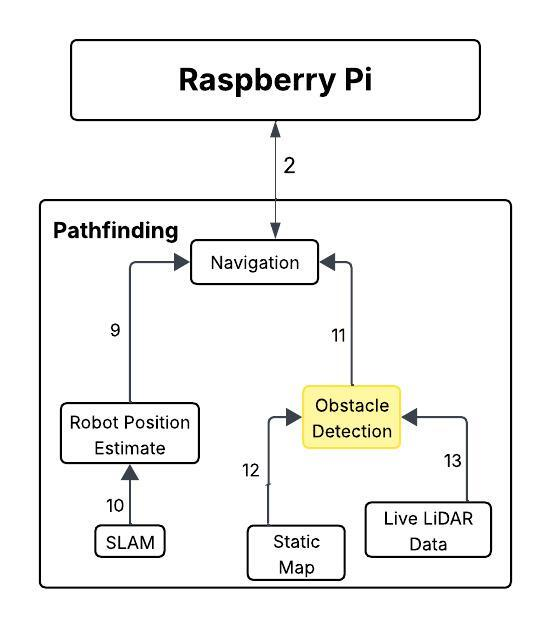
\includegraphics[width=0.60\textwidth]{images/pathfinding 2/Data_Flow_ObstacleD.jpeg}
 \caption{Pathfinding Subsystem - Obstacle Detection} % Be sure to change the caption.
\end{figure}

\subsubsection{Assumptions}
% Any assumptions made in the definition of the subsystem should be listed and described. Pay particular attention to assumptions concerning interfaces and interactions with other layers.
The rover will be able to register static and dynamic obstacles and be detected with LiDAR.
\subsubsection{Responsibilities}
% Each of the responsibilities/features/functions/services of the subsystem as identified in the architectural summary must be expanded to more detailed responsibilities. These responsibilities form the basis for the identification of the finer-grained responsibilities of the layer's internal subsystems. Clearly describe what each subsystem does.

The rover will be able to detect obstacles and update the graph representation Subsystem by marking a cell as untraversable. The obstacle detection subsystem should also be able to be integrated with LiDAR and other sensors. If the close-range sensors get triggered the rover should halt movement and retreat a set distance before reactivating its pathfinding.

The pathfinding algorithm creates a grid using the map the static map subsystem provided, representing the environment with the LiDAR Range. The grid will contain nodes that contain properties such as: 
\begin{itemize}
  \item Traverability (true/false).
  \item Coordinates in world space.
\end{itemize}
\subsubsection{Subsystem Interfaces}
% Each of the inputs and outputs for the subsystem are defined here. Create a table with an entry for each labelled interface that connects to this subsystem. For each entry, describe any incoming and outgoing data elements will pass through this interface.


\begin{table}[H]
\caption{Pathfinding Subsystem - Obstacle Detection} 
\begin{center}
    \begin{tabular}{ | p{1.8cm} | p{8cm} | p{2cm} | p{3cm} |}
    \hline
    ID & Description & Inputs & Outputs  \\ \hline
    \#11 & Algorithm will send a signal to the navigation. & N/A & Marked Obstacles \\ \hline
    \#12 & Algorithm combines the data from map. & Map Data  & N/A \\ \hline
    \#13 & Algorithm combines the data from LiDAR. & Scan Data & N/A \\ \hline
    \end{tabular}
\end{center}
\end{table}


\newpage

\subsection{Navigation Subsystems}
The Navigation Subsystem enables the Roam\_Bot to autonomously navigate the environment by combining real-time position data from the Robot Position Estimate Subsystem with obstacle information from the SLAM-generated map. It generates an optimal path through the terrain, considering both the robot's current pose and the locations of obstacles, and continuously adjusts the path as the environment changes.
%%%%%%%%%%%%%%%%%%%%%%%%%%%%%%%%%%%%%%%%%%%%%%%%%%%%%%%%%%%%%%%%%%%%%%%%%%%%
%   Change the graphic here. Put your image in the 'images' folder
%   and update the name from 'images/test_image' to your image name
\begin{figure}[h!]
	\centering
 	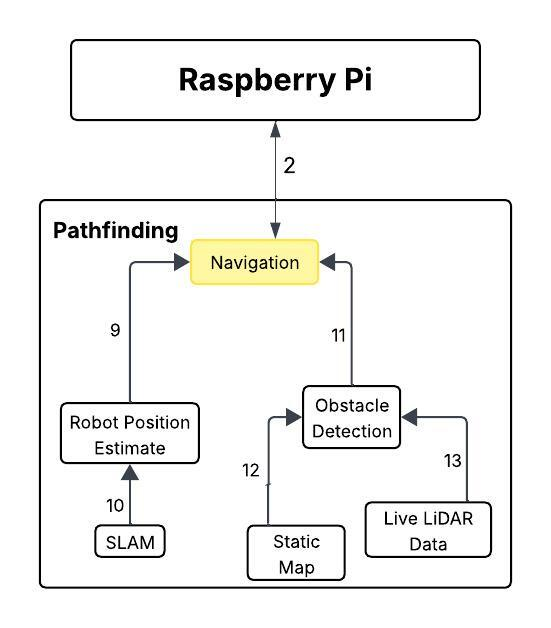
\includegraphics[width=0.60\textwidth]{images/pathfinding 2/Data_Flow_Navigation.jpeg}
 \caption{Pathfinding Subsystem - Navigation} % Be sure to change the caption.
\end{figure}

\subsubsection{Assumptions}
% Any assumptions made in the definition of the subsystem should be listed and described. Pay particular attention to assumptions concerning interfaces and interactions with other layers.

The pathfinding algorithm requires that the graph is already constructed, and LiDAR is active.
\subsubsection{Responsibilities}
% Each of the responsibilities/features/functions/services of the subsystem as identified in the architectural summary must be expanded to more detailed responsibilities. These responsibilities form the basis for the identification of the finer-grained responsibilities of the layer's internal subsystems. Clearly describe what each subsystem does.

The pathfinding algorithm calculates either the optimal or heuristic-based path from a start to end node. The pathfinding algorithms should also allow for multiple algorithms, such as A*, Dijkstra's, Breadth-First-Search, etc. While also handling static and dynamic obstacles.
\subsubsection{Subsystem Interfaces}
% Each of the inputs and outputs for the subsystem are defined here. Create a table with an entry for each labelled interface that connects to this subsystem. For each entry, describe any incoming and outgoing data elements will pass through this interface.

\begin{table}[H]
\caption{Pathfinding Subsystem - Navigation} 
\begin{center}
    \begin{tabular}{ | p{1.8cm} | p{8cm} | p{2cm} | p{3cm} |}
    \hline
    ID & Description & Inputs & Outputs  \\ \hline
    \#2 & Sending movement decision to Raspberry Pi. & N/A & Data to TM4C (Microcontroller) \\ \hline
    \#9 & Receives approximate position odometry. & Position from SLAM & N/A \\ \hline
    \#11 & Receives obstacles detected from scan. & Obstacle Detection & N/A \\ \hline
    \end{tabular}
\end{center}
\end{table}

\newpage


\subsection{Live LiDAR Data Subsystems}
The LiDAR subsystem is implemented as a ROS package that interfaces with and drives the LiDAR hardware module, providing the Roam\_Bot with real time scan data used to perceive and interpret the surrounding terrain.
%%%%%%%%%%%%%%%%%%%%%%%%%%%%%%%%%%%%%%%%%%%%%%%%%%%%%%%%%%%%%%%%%%%%%%%%%%%%
%   Change the graphic here. Put your image in the 'images' folder
%   and update the name from 'images/test_image' to your image name
\begin{figure}[h!]
	\centering
 	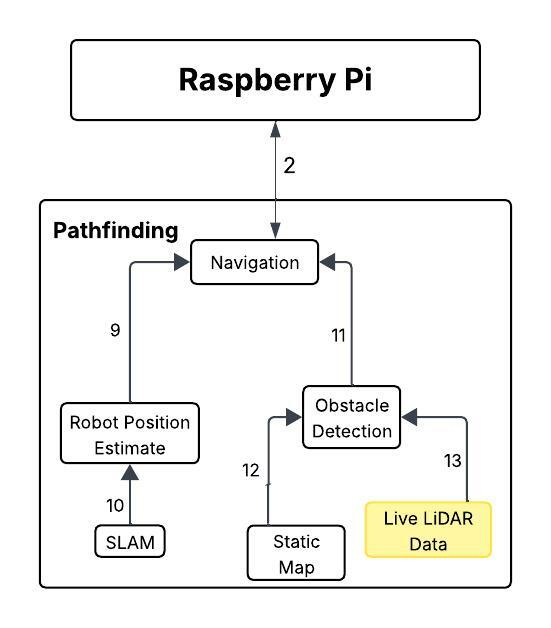
\includegraphics[width=0.60\textwidth]{images/pathfinding 2/Data_Flow_LiveLiDAR.jpeg}
 \caption{Pathfinding Subsystem - Live LiDAR Data} % Be sure to change the caption.
\end{figure}

\subsubsection{Assumptions}
% Any assumptions made in the definition of the subsystem should be listed and described. Pay particular attention to assumptions concerning interfaces and interactions with other layers.
\begin{itemize}
    \item Static Obstacles are Detected Within Range
    \item Robot Operates on a Relatively Flat Plane
    \item Costmap is Regularly Updated with LiDAR Data
    \item No Excessive Sensor Noise or Clutter
\end{itemize}

The LiDAR subsystem requires that the Roam\_Bot be turned on.
\subsubsection{Responsibilities}
% Each of the responsibilities/features/functions/services of the subsystem as identified in the architectural summary must be expanded to more detailed responsibilities. These responsibilities form the basis for the identification of the finer-grained responsibilities of the layer's internal subsystems. Clearly describe what each subsystem does.

The LiDAR subsystem takes the input given by its sensors and sends all relevant information to the Obstacle Detection subsystem, which creates a costmap.

\subsubsection{Subsystem Interfaces}


% Each of the inputs and outputs for the subsystem are defined here. Create a table with an entry for each labelled interface that connects to this subsystem. For each entry, describe any incoming and outgoing data elements will pass through this interface.

\begin {table}[H]
\caption {Pathfinding Subsystem - Live LiDAR Data} 
\begin{center}
    \begin{tabular}{ | p{1cm} | p{6cm} | p{3cm} | p{3cm} |}
    \hline
    ID & Description & Inputs & Outputs \\ \hline
    \#13 &  The LiDAR subsystem will transmit laser scan data to the Obstacle Detection subsystem, which will process the input, convert it into a structured grid, and divide it into individual cells for further analysis.
    & \pbox{3cm}{N/A} & \pbox{3cm}{Obstacle Detection}  \\ \hline
    \end{tabular}
\end{center}
\end{table}

\newpage



\subsection{Robot Position Estimate Subsystem}

The Robot Position Estimate Subsystem is responsible for determining the robot's current pose (position and orientation) within a map generated by SLAM. It continuously updates the pose using LiDAR data and provides this information to the Navigation Decision Subsystem for path planning and movement control.

\begin{figure}[h!]
	\centering
 	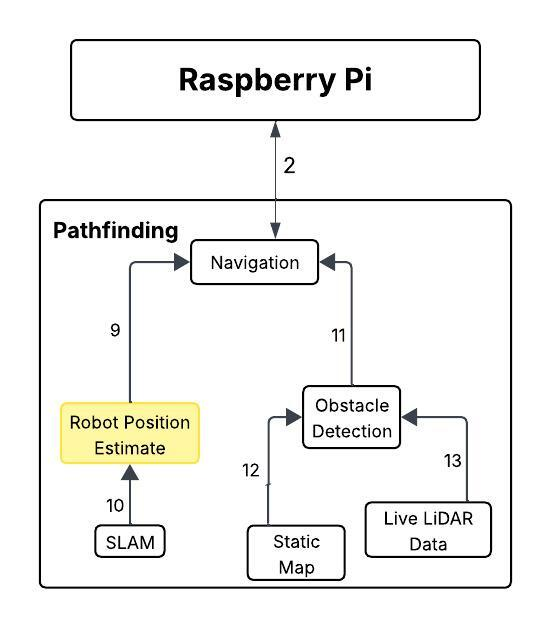
\includegraphics[width=0.80\textwidth]{images/pathfinding 2/Data_Flow_RobotPosition.jpeg}
 	\caption{Pathfinding Subsystem - Position Estimate}
\end{figure}

\subsubsection{Assumptions}

\begin{itemize}
    \item SLAM is functioning correctly and consistently receives LiDAR input.
    \item The robot operates in a primarily static environment suitable for SLAM-based localization.
    \item The initial pose is known or initialized at the origin.
    \item The Raspberry Pi is fully operational and can run SLAM in real time.
\end{itemize}

\subsubsection{Responsibilities}

The Robot Position Estimate Subsystem performs the following functions:
\begin{itemize}
  \item Accepts pose data from the SLAM subsystem.
  \item Maintains the robot’s estimated pose in the global coordinate frame.
  \item Provides updated pose data to the Navigation Decision Subsystem for route planning and motion.
  \item Supports coordinate conversion as necessary for integration with grid-based navigation.
\end{itemize}

\subsubsection{Subsystem Interfaces}

\begin{table}[H]
\caption{Pathfinding Subsystem - Position Estimate}
\begin{center}
    \begin{tabular}{ | p{1.5cm} | p{6cm} | p{3cm} | p{3cm} |}
    \hline
    ID & Description & Inputs & Outputs \\ \hline
    \#9  & Current estimated robot pose for navigation decisions & N/A & Robot Pose\\ \hline
    \#10 & Pose data provided by SLAM & SLAM Pose & N/A \\ \hline
    \end{tabular}
\end{center}
\end{table}

\newpage






\subsection{SLAM}
The SLAM subsystem processes data to simultaneously localize the robot within an environment and build a global occupancy grid map. This enables the Robot Position Estimate Subsystem to determine the robot's real time pose (x, y, θ) in relation to the mapped surroundings, which is critical for accurate navigation and planning.

% This section should be a general description of a particular subsystem for the given layer. For most subsystems, an extract of the architectural block diagram with data flows is useful. This should consist of the subsystem being described and those subsystems with which it communicates.




%%%%%%%%%%%%%%%%%%%%%%%%%%%%%%%%%%%%%%%%%%%%%%%%%%%%%%%%%%%%%%%%%%%%%%%%%%%%
%   Change the graphic here. Put your image in the 'images' folder
%   and update the name from 'images/test_image' to your image name
\begin{figure}[h!]
	\centering
 	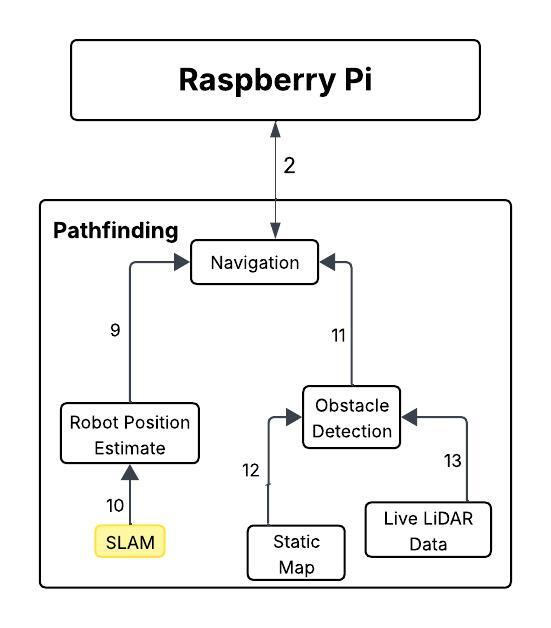
\includegraphics[width=0.80\textwidth]{images/pathfinding 2/Data_Flow_SLAM.jpeg}
 \caption{Pathfinding Subsystem - SLAM} % Be sure to change the caption.
\end{figure}

\subsubsection{Assumptions}
% Any assumptions made in the definition of the subsystem should be listed and described. Pay particular attention to assumptions concerning interfaces and interactions with other layers.
\begin{itemize}
    \item ROS2 Jazzy is installed on the Raspberry Pi 5.
    \item Nav2 Jazzy is installed on the Raspberry Pi 5.
    \item The Static Map is locatable on the Raspberry Pi 5.
    \item Robot operates on a relatively flat plane.
\end{itemize}
\subsubsection{Responsibilities}
% Each of the responsibilities/features/functions/services of the subsystem as identified in the architectural summary must be expanded to more detailed responsibilities. These responsibilities form the basis for the identification of the finer-grained responsibilities of the layer's internal subsystems. Clearly describe what each subsystem does.

The responsibilites that SLAM uses is:
\begin{itemize}
  \item Real-Time Map Building: (Mapping) Continuously generates a 2D or 3D map of the environment based on sensor data (typically LiDAR or depth camera).
  \item Robot Localization: Estimates the robot's pose (x, y, θ) in the global map frame in real time. Uses scan matching or visual feature matching to align sensor data with the evolving map.
\end{itemize}
\subsubsection{Subsystem Interfaces}
% Each of the inputs and outputs for the subsystem are defined here. Create a table with an entry for each labelled interface that connects to this subsystem. For each entry, describe any incoming and outgoing data elements will pass through this interface.

\begin {table}[H]
\caption {Pathfinding Subsystem - SLAM} 
\begin{center}
    \begin{tabular}{ | p{1.2cm} | p{6cm} | p{3cm} | p{3cm} |}
    \hline
    ID & Description & Inputs & Outputs \\ \hline
    \#10 & Slam's localization function outputs the robot's position estimate & \pbox{3cm}{N/A} & \pbox{3cm}{SLAM Pose}  \\ \hline

    \end{tabular}
\end{center}
\end{table}
\newpage
\section{Interface Subsystems}
The interface subsystems are responsible for getting user input and translating it to the motion of the rover.

\subsection{User Interface}
This is the user interface, where users will be able to input which path-finding algorithm they want the rover to utilize, and control the motion of the rover.

\begin{figure}[h!]
	\centering
 	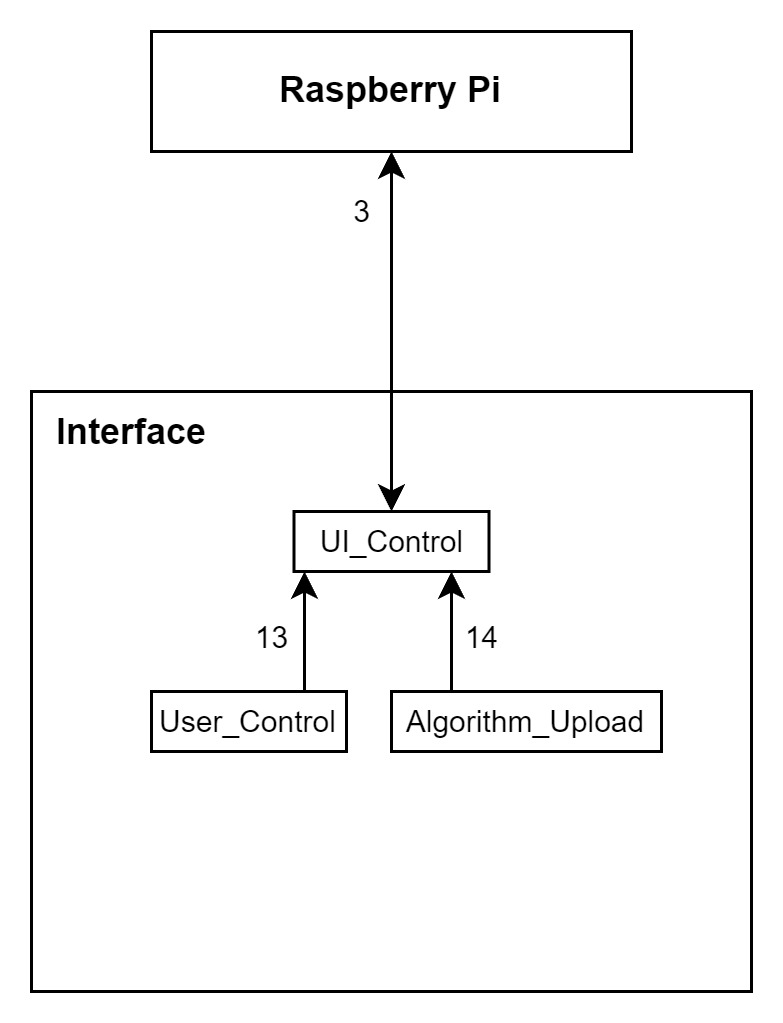
\includegraphics[width=0.45\textwidth]{images/interface/interface.jpg}
 \caption{Interface Subsystem} % Be sure to change the caption
\end{figure}

%%%%%%%%%%%%%%%%%%%%%%%%%%%%%%%%%%%%%%%%%%%%%%%%%%%%%%%%%%%%%%%%%%%%%%%%%%%%
%   Change the graphic here. Put your image in the 'images' folder
%   and update the name from 'images/test_image' to your image name

%\begin{figure}[h!]
	%\centering
 	%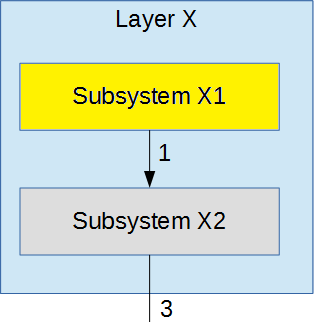
\includegraphics[width=0.60\textwidth]{images/subsystem}
 %\caption{Example subsystem description diagram} % Be sure to change the caption.
%\end{figure}


\subsubsection{Assumptions}
We are assuming that the user will be able to utilize the UI. We will be printing out specific instructions, and cover for any possible cases.

\subsubsection{Responsibilities}
It should be user-friendly and easy to use, so that users can simply run the program and send commands to the rover.

\subsubsection{Subsystem Interfaces}
%Each of the inputs and outputs for the subsystem are defined here. Create a table with an entry for each labelled interface that connects to this subsystem. For each entry, describe any incoming and outgoing data elements will pass through this interface.

\begin {table}[H]
\caption {Interface Subsystem} 
\begin{center}
    \begin{tabular}{ | p{1cm} | p{6cm} | p{3cm} | p{3cm} |}
    \hline
    ID & Description & Inputs & Outputs \\ \hline
    \#3 & UI & \pbox{3cm}{N/A} & \pbox{3cm}{Screen}  \\ \hline
    \#13 & User Control & \pbox{3cm}{Speed \\ Direction} & \pbox{3cm}{Motion}  \\ \hline
    \#14 & Algorithm Upload & \pbox{3cm}{Algorithm Name} & \pbox{3cm}{Path-finding}  \\ \hline
    
    \end{tabular}
\end{center}
\end{table}

%\subsection{Subsystem 2}
%Repeat for each subsystem

%\subsection{Subsystem 3}
%Repeat for each subsystem


\newpage

%%% References
%\bibliographystyle{plain}
\bibliographystyle{reference/IEEEtran_custom}
\bibliography{reference/refs}{}

\end{document}